\documentclass[a4paper,12pt]{article}

\usepackage[utf8x]{inputenc}
\usepackage[T2A]{fontenc}
\usepackage[english, russian]{babel}

% Опционно, требует  apt-get install scalable-cyrfonts.*
% и удаления одной строчки в cyrtimes.sty
% Сточку не удалять!
% \usepackage{cyrtimes}

% Картнки и tikz
\usepackage{graphicx}
\usepackage{tikz}
\usetikzlibrary{snakes,arrows,shapes}


% Некоторая русификация.
\usepackage{misccorr}
\usepackage{indentfirst}
\renewcommand{\labelitemi}{\normalfont\bfseries{--}}

% Увы, поля придётся уменьшить из-за листингов.
\topmargin -1cm
\oddsidemargin -0.5cm
\evensidemargin -0.5cm
\textwidth 17cm
\textheight 24cm

\sloppy

% Оглавление в PDF
\usepackage[
bookmarks=true,
colorlinks=true, linkcolor=black, anchorcolor=black, citecolor=black, menucolor=black,filecolor=black, urlcolor=black,
unicode=true
]{hyperref}

% Для исходного кода в тексте
\newcommand{\Code}[1]{\texttt{#1}}

\usepackage{verbatim}
\usepackage{fancyvrb}
\fvset{frame=leftline, fontsize=\small, framerule=0.4mm, rulecolor=\color{darkgray}, commandchars=\\\{\}}
\renewcommand{\theFancyVerbLine}{\small\arabic{FancyVerbLine}}


\title{Отчёт по лабораторной работе \\ <<Динамическая IP-маршрутизация>>}
\author{Зиновьев Д.В., ИУ7-32м}

\begin{document}

\maketitle

\tableofcontents

\section{Настройка сети}

\subsection{Топология сети}

Топология сети и используемые IP-адреса показаны на рисунке~\ref{fig:network}.

\begin{figure}
\centering
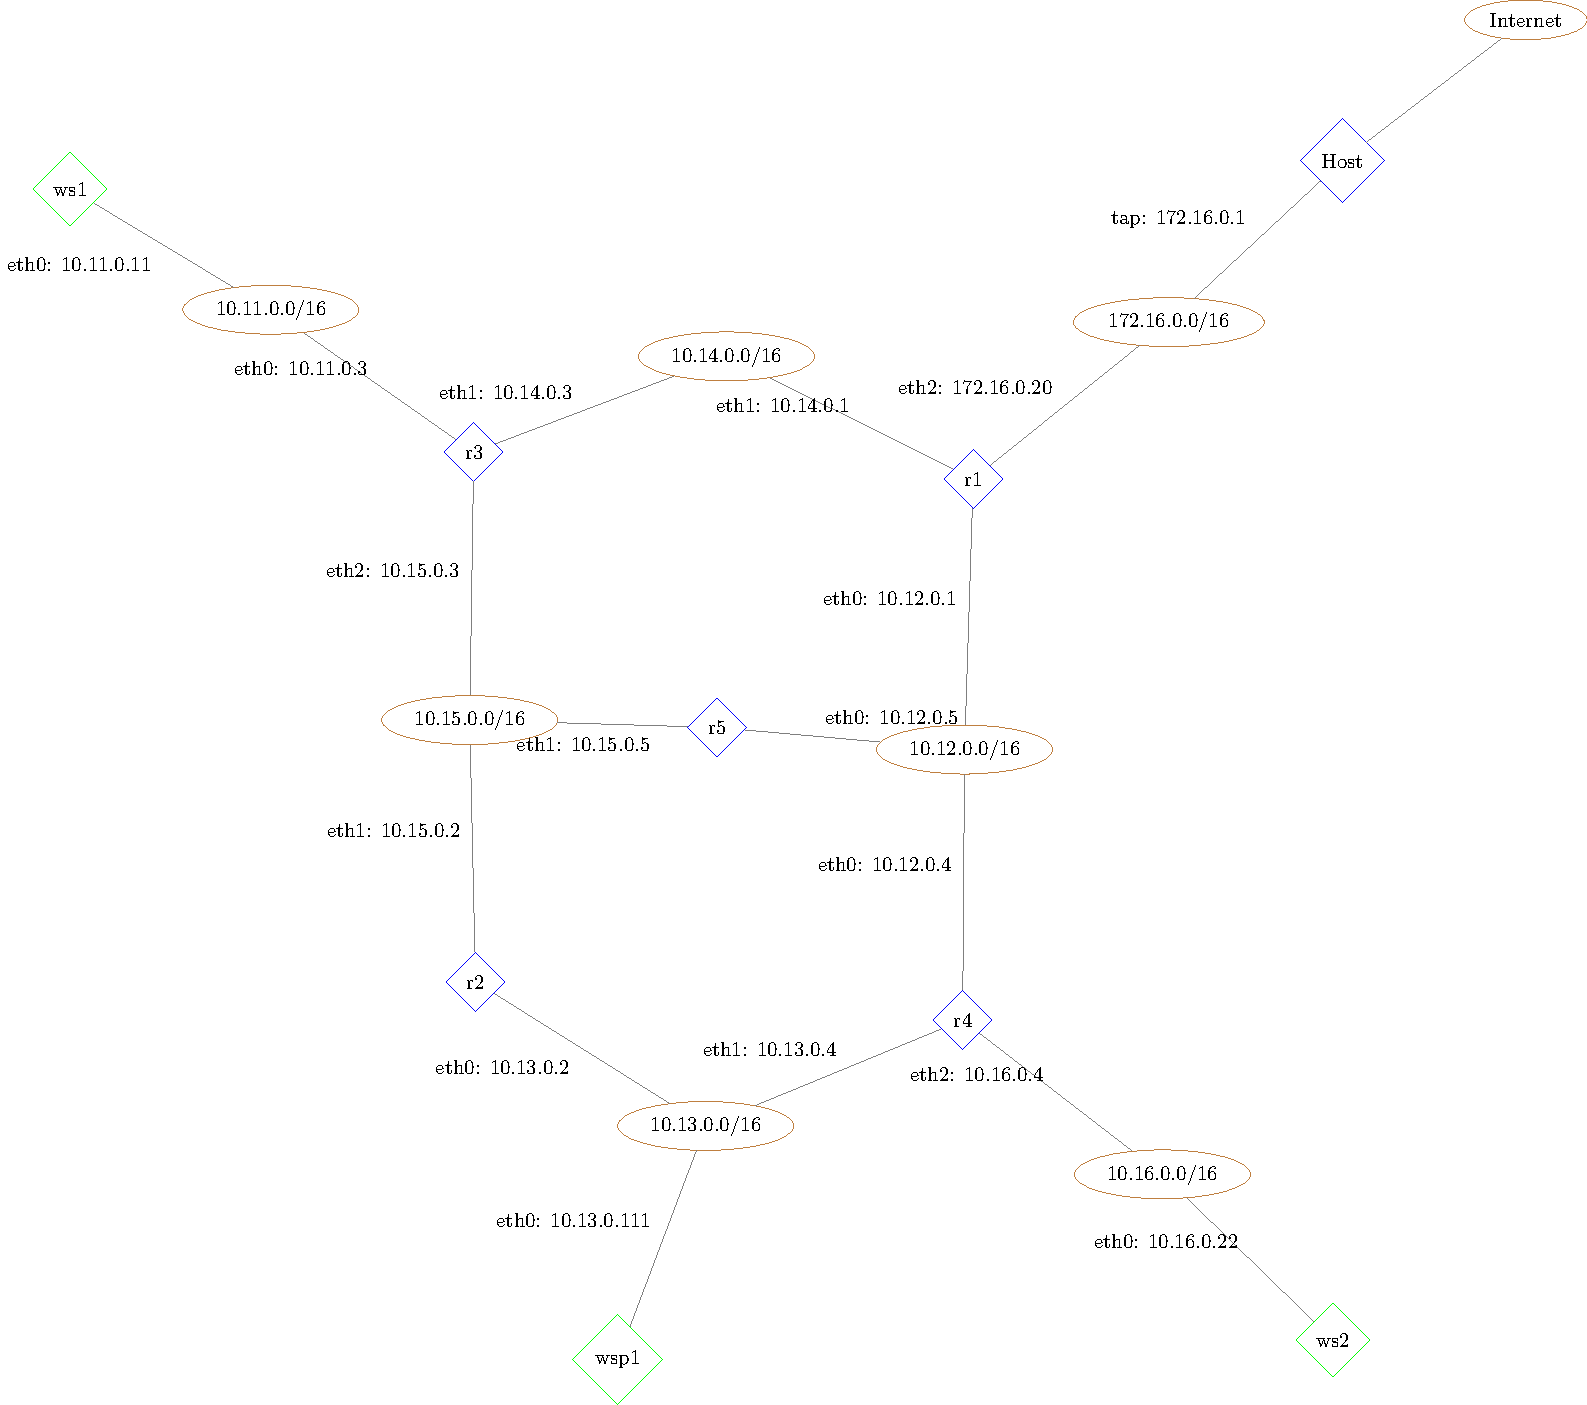
\includegraphics[width=0.8\textwidth]{includes/network_gv.pdf}
\caption{Топология сети}
\label{fig:network}
\end{figure}

Перечень узлов, на которых используется динамическая IP-маршрутизация: \textbf{r1} - \textbf{r5}, \textbf{wsp1}.


\subsection{Назначение IP-адресов}

Ниже приведён файл сетевой настройки  маршрутизатора \textbf{r3}.

\begin{Verbatim}
r3:~# cat /etc/network/interfaces 
auto lo
iface lo inet loopback

auto eth0
iface eth0 inet static
address 10.11.0.3
netmask 255.255.0.0

auto eth1
iface eth1 inet static
address 10.14.0.3
netmask 255.255.0.0

auto eth2
iface eth2 inet static
address 10.15.0.3
netmask 255.255.0.0
\end{Verbatim}

Ниже приведён файл сетевой настройки рабочей станции \textbf{ws1}.

\begin{Verbatim}
ws1:~# cat /etc/network/interfaces 
auto lo
iface lo inet loopback

auto eth0
iface eth0 inet static
address 10.11.0.11
netmask 255.255.0.0
gateway 10.11.0.3
\end{Verbatim}


\subsection{Настройка протокола RIP}

Ниже приведен файл \Code{/etc/quagga/ripd.conf} маршрутизатора \textbf{r5}.

\begin{Verbatim}
r5:~# cat /etc/quagga/ripd.conf
router rip

network eth0
network eth1

timers basic 10 60 120

redistribute kernel
redistribute connected

log file /var/log/quagga/ripd.log
\end{Verbatim}


Ниже приведен файл \Code{/etc/quagga/ripd.conf} рабочий станции, связанной с несколькими маршрутизаторами \textbf{wsp1}.

\begin{Verbatim}
wsp1:~# cat /etc/quagga/ripd.conf
router rip

network eth0

timers basic 10 60 120

redistribute kernel
redistribute connected

log file /var/log/quagga/ripd.log
\end{Verbatim}


\section{Проверка настройки протокола RIP}

Вывод \textbf{traceroute} от \textbf{ws1} до \textbf{ws2} при нормальной работе сети.

\begin{Verbatim}
ws1:~# traceroute 10.16.0.22
traceroute to 10.16.0.22 (10.16.0.22), 64 hops max, 40 byte packets
 1  10.11.0.3 (10.11.0.3)  1 ms  0 ms  0 ms
 2  10.15.0.5 (10.15.0.5)  19 ms  0 ms  0 ms
 3  10.13.0.4 (10.13.0.4)  11 ms  0 ms  0 ms
 4  10.16.0.22 (10.16.0.22)  9 ms  0 ms  0 ms
\end{Verbatim}

Вывод \textbf{traceroute} от узла \textbf{wsp1} до внешнего IP (195.19.38.2).

\begin{Verbatim}
wsp1:~# traceroute 195.19.38.2
traceroute to 195.19.38.2 (195.19.38.2), 64 hops max, 40 byte packets
 1  10.13.0.4 (10.13.0.4)  8 ms  0 ms  0 ms
 2  10.12.0.1 (10.12.0.1)  12 ms  0 ms  0 ms
 3  172.16.0.1 (172.16.0.1)  15 ms  0 ms  0 ms
 4  * * *
\end{Verbatim}

Вывод сообщения RIP.

\begin{Verbatim}
r3:~# tcpdump -ntve -i any dst 224.0.0.9
tcpdump: listening on any, link-type LINUX_SLL (Linux cooked), capture size 96 bytes
  M fa:de:dc:30:96:57 ethertype IPv4 (0x0800), length 128: (tos 0x0, ttl 1, id 0, offset 0,
      flags [DF], proto UDP (17), length 112) 10.14.0.1.520 > 224.0.0.9.520: 
	RIPv2, Response, length: 84, routes: 4
	  AFI: IPv4:       10.12.0.0/16, tag 0x0000, metric: 1, next-hop: self
	  AFI: IPv4:       10.13.0.0/16, tag 0x0000, metric: 2, next-hop: self[|rip]
\end{Verbatim}

Вывод таблицы RIP.

\begin{Verbatim}
r3# show ip rip
Codes: R - RIP, C - connected, S - Static, O - OSPF, B - BGP
Sub-codes:
      (n) - normal, (s) - static, (d) - default, (r) - redistribute,
      (i) - interface

     Network            Next Hop         Metric From            Tag Time
C(i) 10.11.0.0/16       0.0.0.0               1 self              0
R(n) 10.12.0.0/16       10.15.0.5             2 10.15.0.5         0 00:56
R(n) 10.13.0.0/16       10.15.0.2             2 10.15.0.2         0 00:56
C(i) 10.14.0.0/16       0.0.0.0               1 self              0
C(i) 10.15.0.0/16       0.0.0.0               1 self              0
R(n) 10.16.0.0/16       10.15.0.5             3 10.15.0.5         0 00:56
\end{Verbatim}

Вывод таблицы маршрутизации.

\begin{Verbatim}
r3:~# ip r
10.16.0.0/16 via 10.15.0.5 dev eth2  proto zebra  metric 3 
10.11.0.0/16 dev eth0  proto kernel  scope link  src 10.11.0.3 
10.14.0.0/16 dev eth1  proto kernel  scope link  src 10.14.0.3 
10.15.0.0/16 dev eth2  proto kernel  scope link  src 10.15.0.3 
10.12.0.0/16 via 10.15.0.5 dev eth2  proto zebra  metric 2 
10.13.0.0/16 via 10.15.0.2 dev eth2  proto zebra  metric 2
\end{Verbatim}

\section{Расщепленный горизонт и испорченные обратные обновления}

Вывод сообщения RIP при split horizon.

\begin{Verbatim}
r3:~# tcpdump -ntve -s 0 -i eth2 src 10.15.0.3 and dst 224.0.0.9
tcpdump: listening on eth2, link-type EN10MB (Ethernet), capture size 65535 bytes
c2:57:e2:f3:3f:00 > 01:00:5e:00:00:09, ethertype IPv4 (0x0800), length 86: (tos 0x0, ttl 1, id 0, offset 0,
    flags [DF], proto UDP (17), length 72) 10.15.0.3.520 > 224.0.0.9.520: 
	RIPv2, Response, length: 44, routes: 2
	  AFI: IPv4:       10.11.0.0/16, tag 0x0000, metric: 1, next-hop: self
	  AFI: IPv4:       10.14.0.0/16, tag 0x0000, metric: 1, next-hop: self
\end{Verbatim}

Вывод сообщения RIP при split horizon + poisoned reverse.

\begin{Verbatim}
r3:~# tcpdump -ntve -s 0 -i eth2 src 10.15.0.3 and dst 224.0.0.9
tcpdump: listening on eth2, link-type EN10MB (Ethernet), capture size 65535 bytes
c2:57:e2:f3:3f:00 > 01:00:5e:00:00:09, ethertype IPv4 (0x0800), length 166: (tos 0x0, ttl 1, id 0, offset 0,
    flags [DF], proto UDP (17), length 152) 10.15.0.3.520 > 224.0.0.9.520: 
	RIPv2, Response, length: 124, routes: 6
	  AFI: IPv4:       10.11.0.0/16, tag 0x0000, metric: 1, next-hop: self
	  AFI: IPv4:       10.12.0.0/16, tag 0x0000, metric: 2, next-hop: self
	  AFI: IPv4:       10.13.0.0/16, tag 0x0000, metric: 16, next-hop: 10.15.0.2
	  AFI: IPv4:       10.14.0.0/16, tag 0x0000, metric: 1, next-hop: self
	  AFI: IPv4:       10.15.0.0/16, tag 0x0000, metric: 16, next-hop: self
	  AFI: IPv4:       10.16.0.0/16, tag 0x0000, metric: 3, next-hop: self
\end{Verbatim}

Вывод сообщения RIP без split horizon.

\begin{Verbatim}
r3:~# tcpdump -ntve -s 0 -i eth2 src 10.15.0.3 and dst 224.0.0.9
tcpdump: listening on eth2, link-type EN10MB (Ethernet), capture size 65535 bytes
c2:57:e2:f3:3f:00 > 01:00:5e:00:00:09, ethertype IPv4 (0x0800), length 146: (tos 0x0, ttl 1, id 0, offset 0,
    flags [DF], proto UDP (17), length 132) 10.15.0.3.520 > 224.0.0.9.520: 
	RIPv2, Response, length: 104, routes: 5
	  AFI: IPv4:       10.12.0.0/16, tag 0x0000, metric: 2, next-hop: self
	  AFI: IPv4:       10.13.0.0/16, tag 0x0000, metric: 2, next-hop: 10.15.0.2
	  AFI: IPv4:       10.14.0.0/16, tag 0x0000, metric: 1, next-hop: self
	  AFI: IPv4:       10.15.0.0/16, tag 0x0000, metric: 1, next-hop: self
	  AFI: IPv4:       10.16.0.0/16, tag 0x0000, metric: 3, next-hop: self
\end{Verbatim}


\section{Имитация устранимой поломки в сети}

Вывод \textbf{traceroute} от \textbf{wsp1} до \textbf{r3}.

\begin{Verbatim}
wsp1:~# traceroute 10.14.0.3
traceroute to 10.14.0.3 (10.14.0.3), 64 hops max, 40 byte packets
 1  10.13.0.2 (10.13.0.2)  10 ms  0 ms  0 ms
 2  10.14.0.3 (10.14.0.3)  10 ms  0 ms  0 ms
\end{Verbatim}

Выключаем маршрутизатор \textbf{r2}.

Устаревание в таблицы протокола RIP на \textbf{r3}.

\begin{Verbatim}
r3# show ip rip
Codes: R - RIP, C - connected, S - Static, O - OSPF, B - BGP
Sub-codes:
      (n) - normal, (s) - static, (d) - default, (r) - redistribute,
      (i) - interface

     Network            Next Hop         Metric From            Tag Time
C(i) 10.11.0.0/16       0.0.0.0               1 self              0
R(n) 10.12.0.0/16       10.15.0.5             2 10.15.0.5         0 00:00
R(n) 10.13.0.0/16       10.15.0.2             2 10.15.0.2         0 00:01
C(i) 10.14.0.0/16       0.0.0.0               1 self              0
C(i) 10.15.0.0/16       0.0.0.0               1 self              0
R(n) 10.16.0.0/16       10.15.0.2             3 10.15.0.2         0 00:01
\end{Verbatim}

Перестроенная таблица RIP на \textbf{r3}.

\begin{Verbatim}
r3# show ip rip
Codes: R - RIP, C - connected, S - Static, O - OSPF, B - BGP
Sub-codes:
      (n) - normal, (s) - static, (d) - default, (r) - redistribute,
      (i) - interface

     Network            Next Hop         Metric From            Tag Time
C(i) 10.11.0.0/16       0.0.0.0               1 self              0
R(n) 10.12.0.0/16       10.14.0.1             2 10.14.0.1         0 00:55
R(n) 10.13.0.0/16       10.14.0.1             3 10.14.0.1         0 00:55
C(i) 10.14.0.0/16       0.0.0.0               1 self              0
C(i) 10.15.0.0/16       0.0.0.0               1 self              0
R(n) 10.16.0.0/16       10.14.0.1             3 10.14.0.1         0 00:55
\end{Verbatim}


Вывод \textbf{traceroute} от \textbf{wsp1} до \textbf{r3} после того, как служба RIP перестроила таблицы маршрутизации.

\begin{Verbatim}
wsp1:~# traceroute 10.14.0.3
traceroute to 10.14.0.3 (10.14.0.3), 64 hops max, 40 byte packets
 1  10.13.0.4 (10.13.0.4)  0 ms  0 ms  0 ms
 2  10.12.0.1 (10.12.0.1)  0 ms  1 ms  1 ms
 3  10.14.0.3 (10.14.0.3)  26 ms  1 ms  0 ms
\end{Verbatim}

\section{Имитация неустранимой поломки в сети}

Выключаем \textbf{r3} - теперь сеть 10.11.0.0/16 недостижима.

\begin{Verbatim}
r4:~# tcpdump -ntve -i any -s 0 dst 224.0.0.9
tcpdump: listening on any, link-type LINUX_SLL (Linux cooked), capture size 65535 bytes
Out 4a:e4:d9:3b:f2:04 ethertype IPv4 (0x0800), length 108: (tos 0x0, ttl 1, id 0,
    offset 0, flags [DF], proto UDP (17), length 92) 10.12.0.4.520 > 224.0.0.9.520: 
	RIPv2, Response, length: 64, routes: 3
	  AFI: IPv4:       10.11.0.0/16, tag 0x0000, metric: 16, next-hop: self
	  AFI: IPv4:       10.13.0.0/16, tag 0x0000, metric: 1, next-hop: self
	  AFI: IPv4:       10.16.0.0/16, tag 0x0000, metric: 1, next-hop: self
\end{Verbatim}

\end{document}
